\documentclass[aspectratio=43]{beamer}
\usepackage{amsmath}
\usepackage{amsthm}
\usepackage{mathtools}
\usepackage{csquotes}
\usepackage{tcolorbox}
\usepackage{pstricks}
\usepackage[backend=biber, bibstyle=nature, sorting=nty, citestyle=numeric-comp]{biblatex} %Custom bibliography
\addbibresource{references.bib} %Load references

\useoutertheme{infolines}
\useinnertheme{rectangles}
\usefonttheme{professionalfonts}

\usepackage{pgfplots}
\pgfplotsset{compat=newest}
\usepgfplotslibrary{groupplots}
\usepgfplotslibrary{dateplot}
\usepackage{tikzscale}


\definecolor{orange}{HTML}{f28165}
\definecolor{gray}{HTML}{303030}
\definecolor{yellow}{HTML}{f0be52}
\definecolor{lightorange}{HTML}{f19e58}

\newcommand{\real}{\mathbb{R}} % real numbers
\DeclarePairedDelimiterX{\norm}[1]{\lVert}{\rVert}{#1}
\DeclareMathOperator{\rank}{rank}
\DeclareMathOperator{\bc}{bc}


\makeatletter
\newcommand{\mybox}[1]{%
	\setbox0=\hbox{#1}%
	\setlength{\@tempdima}{\dimexpr\wd0+13pt}%
	\begin{tcolorbox}[colback=orange,colframe=orange,boxrule=0.5pt,arc=4pt,
		left=6pt,right=6pt,top=6pt,bottom=6pt,boxsep=0pt,width=\@tempdima]
		\textcolor{white}{#1}
	\end{tcolorbox}
}
\makeatother

\newtheorem{thm}{Theorem}[section]
%\newtheorem{proof}[thm]{Proof}
%\newtheorem{lemma}[thm]{Lemma}
\newtheorem{rem}[thm]{Remark}
\newtheorem{cor}[thm]{Corollary}
\newtheorem{ex}[thm]{Example}
\newtheorem{assu}[thm]{Assumption}
\newtheorem{alg}[thm]{Algorithm}
\newtheorem{defn}[thm]{Definition}

\usecolortheme[named=orange]{structure}
\usecolortheme{sidebartab}
\usecolortheme{orchid}
\usecolortheme{whale}
\setbeamercolor{alerted text}{fg=yellow}
\setbeamercolor{block title alerted}{bg=alerted text.fg!90!black}
\setbeamercolor{block title example}{bg=lightorange!60!black}
\setbeamercolor{background canvas}{bg=white}
\setbeamercolor{normal text}{bg=white,fg=black}

\setbeamertemplate{footline}
{
	\leavevmode%
	\hbox{%
		\begin{beamercolorbox}[wd=.333333\paperwidth,ht=2.25ex,dp=1ex,center]{author in head/foot}%
			\usebeamerfont{author in head/foot}\insertshortauthor~~(\insertshortinstitute)
		\end{beamercolorbox}%
		\begin{beamercolorbox}[wd=.333333\paperwidth,ht=2.25ex,dp=1ex,center]{title in head/foot}%
			\usebeamerfont{title in head/foot}\insertshorttitle
		\end{beamercolorbox}%
		\begin{beamercolorbox}[wd=.333333\paperwidth,ht=2.25ex,dp=1ex,center]{date in head/foot}%
			\usebeamerfont{date in head/foot}\insertshortdate{}%\hspace*{2em}
			
			%#turning the next line into a comment, erases the frame numbers
			\insertframenumber{} / \inserttotalframenumber\hspace*{2ex} 
			
	\end{beamercolorbox}}%
	\vskip0pt%
}


\setbeamertemplate{blocks}[rectangle]

\setbeamertemplate{section page}
{
	\begin{centering}
		\begin{beamercolorbox}[sep=27pt,center]{part title}
			\usebeamerfont{section title}\insertsection\par
			\usebeamerfont{subsection title}\insertsubsection\par
		\end{beamercolorbox}
	\end{centering}
}

%\setbeamertemplate{subsection page}
%{
%	\begin{centering}
%		\begin{beamercolorbox}[sep=12pt,center]{part title}
%			\usebeamerfont{subsection title}\insertsubsection\par
%		\end{beamercolorbox}
%	\end{centering}
%}

\newcommand{\hlight}[1]{\colorbox{violet!50}{#1}}
\newcommand{\hlighta}[1]{\colorbox{red!50}{#1}}

\usepackage[english]{babel}
\title[Nonnegative Matrix Factorization]{The Why and How of Nonnegative Matrix Factorization} %->->->->-> Check hyperref title <-<-<-<-<-
\subtitle{Topic Presentation}
\author[Group 2]{Group 2 --- Aurélie de Borman, Jennifer Leclipteur, Gilles Peiffer, and Minh-Phuong Tran}
\institute[LINMA2380]{
    LINMA2380 --- Matrix computations
} %You can change the Institution if you are from somewhere else
\date{December 10, 2020}
%\logo{\includegraphics[width= 0.2\textwidth]{images/a-logo.png}}

\begin{document}
    
    \frame{\titlepage}
        
    \section{What: Introduction}
    \begin{frame}{Summary}
    \textbf{Use} : Analysis of high-dimensional data by automatically extracts sparse and meaningful features from a set of nonnegative data vectors\\
    ~\\
    %\begin{figure}
     %   \centering
      %  \includegraphics[width=2cm]{face_image.png}
    %\end{figure}
    %Data matrix : $X\in\real^{p\times n}_+$\\
    \begin{enumerate}
        \item What : Definitions as introduction
        \item Why : Applications
        \item How : Formal view and algorithmic difficulties
        \item What next : Connections to other problems %in Mathematics and Computer Science
        \item Conclusion
    \end{enumerate}
\end{frame}

\begin{frame}{What : Definitions and properties}
     Nonnegative matrix factorization (NMF) is a Linear dimensionality reduction (LDR) \\
         ~\\
         % introduced by Paatero and Tapper in 1994 and more developped by Lee and Seung in 1999
         

     \textbf{NMF} : decomposing a given nonnegative data matrix $X$ as $X \approx W H$ where $W \geq 0$ and $H \geq 0$ %component-wise nonnegative
     
          ~\\
          
     \textbf{LDR} : \\
     \begin{itemize}
         \item From a set of data points $x_j \in R^{p}$ for $1 \leq j \leq n$ 
         \item To a set of dimension $r < min(p,n)$
         \item Thanks to $w_k \in R^p$ for $1 \leq k \leq r$
         \item Such that : $\forall j, x_j \approx \sum_{k = 1}^{r} w_{k} h_{j}(k)$, for some weights $h_j\in R^r$
     \end{itemize}
              ~\\
     Equivalent to \textbf{low-rank matrix approximation} : $X \approx W H$\\
     
     \centering
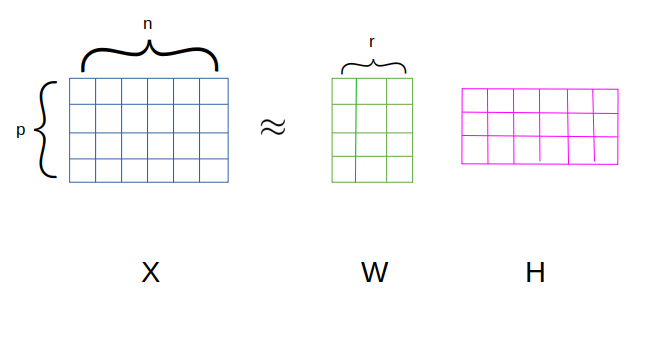
\includegraphics[scale=0.28]{../images/matrices.png}

%     \begin{itemize}
 %    \item $X \in R^{p \times n}$ : $X(:,j) = x_j$ for $1 \leq j \leq n$ %each column of the matrix $X \in R^{p x n}$ is a data point
  %   \item $W \in R^{p \times r}$ : $W(:,k) = w_k$ for $1 \leq k \leq r$ %each column of the matrix $W \in R^{p x r}$ is a basis element
   %  \item $H \in R^{r \times n}$ : $H(:,j) = h_j$ for $1 \leq j \leq n$ %each column of the matrix H gives the coordinates of a data point X(:,j) in the basis W
    % \end{itemize}

\end{frame}

	\section{Why: Applications}
    \begin{frame}{Applications - Image processing}
    \textbf{Goal} : Facial Feature Extraction\\
    ~\\
    \begin{figure}
        \centering
        \includegraphics[width=2cm]{../images/face_image.png}
    \end{figure}
    Data matrix : $X\in\real^{p\times n}_+$\\
    \begin{itemize}
        \item $p$ : total number of pixels
        \item $n$ : number of faces
        \item $X(i,j)$ : the gray-level of the $i$-th pixel in the $j$-th face
    \end{itemize}
\end{frame}
    
\begin{frame}{Applications - Image processing}
    \begin{figure}
        \centering
        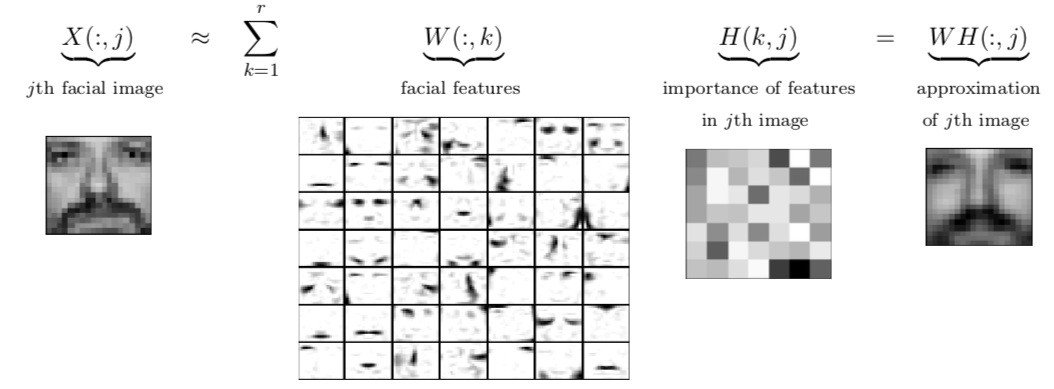
\includegraphics[width=\linewidth]{../images/NMF_app1.png}
    \end{figure}
\end{frame}

\begin{frame}{Applications - Image processing}
    \begin{figure}[h!]
        \centering
        \begin{minipage}{0.45\textwidth}
            \centering
            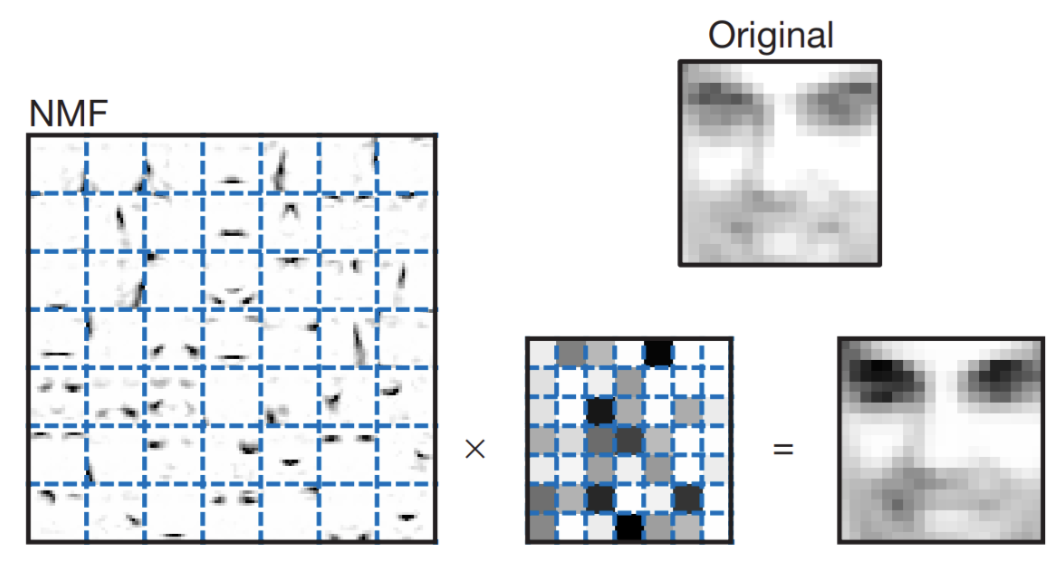
\includegraphics[width=5.3cm]{../images/NMFcomp.png}
            %\caption{NMF decomposition}
            NMF decomposition
        \end{minipage}
        \hfill
        \begin{minipage}{0.45\textwidth}
            \centering
            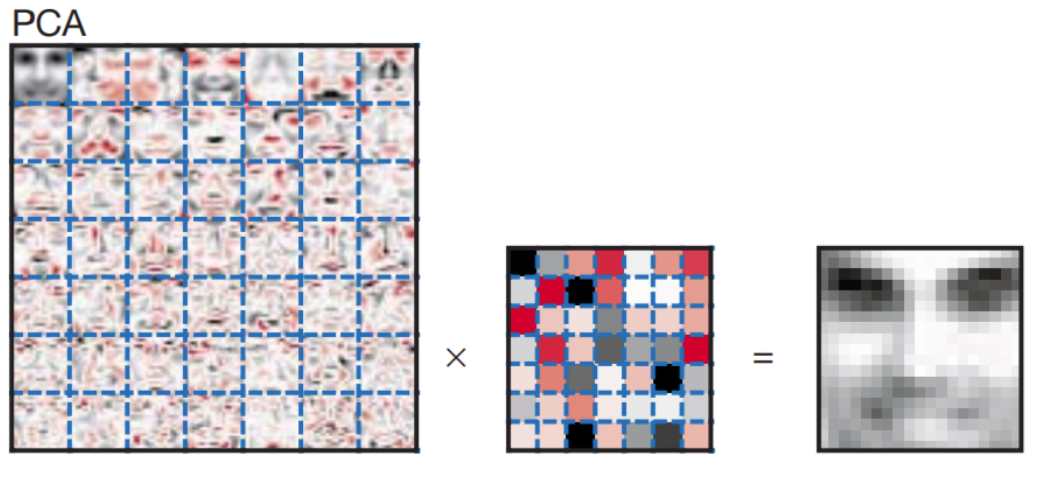
\includegraphics[width=5.5cm]{../images/PCAcomp.png}
            %\caption{PCA decomposition}
            PCA decompostion
        \end{minipage}
    \end{figure}
\end{frame}
\begin{frame}{Applications - Text Mining}
    \textbf{Goal} : Topic Recovery and Document Classification\\
    \vspace{0.7cm}
    Data matrix : $X\in\real^{n\times m}_+$\\
    \begin{itemize}
        \item each column : a document
        \item each line : a word
        \item $X(i,j)$ : number of times the $i$-th word appears in the $j$-th document
    \end{itemize}
    \begin{figure}
        \centering
        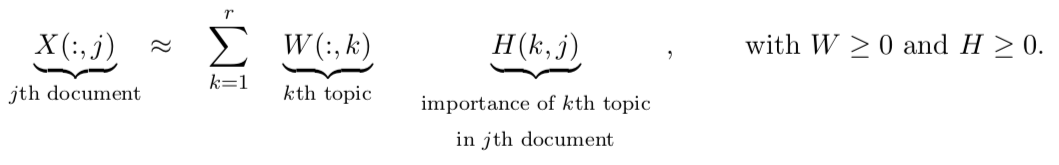
\includegraphics[width=0.9\linewidth]{../images/NMF_app2.png}
    \end{figure}
\end{frame}
\begin{frame}{Applications - Hyperspectral Unmixing}
    \textbf{Goal} :
    \begin{enumerate}
        \item Identify the constitutive materials present in an image
        \item Classify the pixels according to their constitutive materials
    \end{enumerate}
    \vspace{1cm}
    Spectral signature of a pixel: fraction of incident light being reflected by that pixel at different wavelengths\\
\end{frame}

\begin{frame}{Applications - Hyperspectral Unmixing}
    Data matrix : $X\in\real^{n\times m}$\\
    \begin{itemize}
        \item each column : spectral signature of a pixel
    \end{itemize}
    \begin{figure}
        \centering
        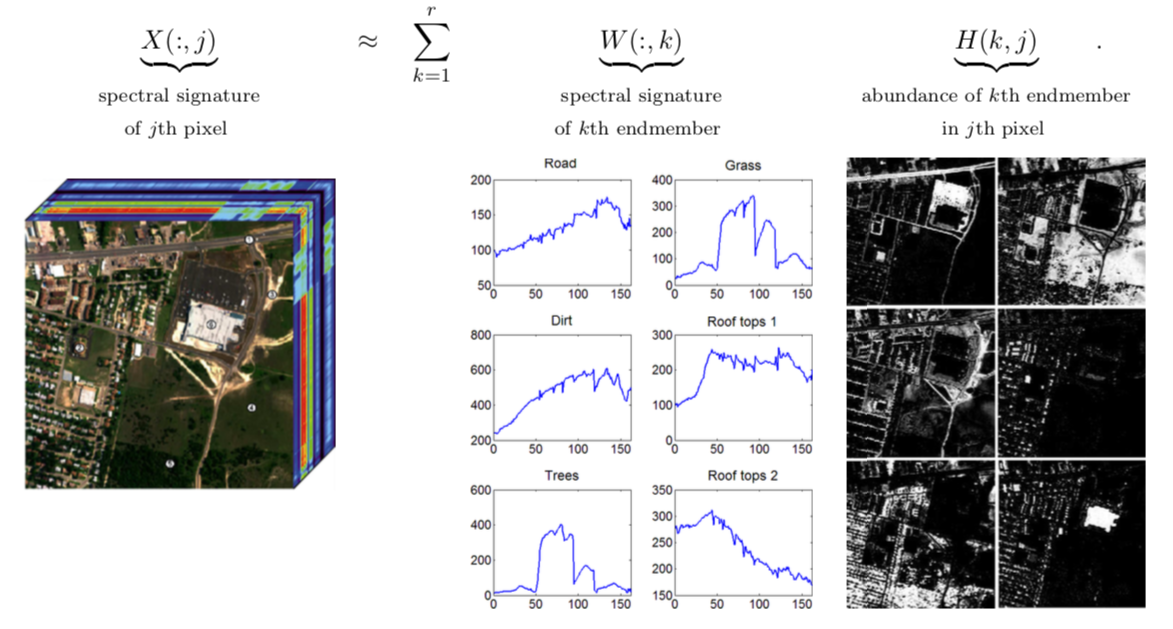
\includegraphics[width=0.85\linewidth]{../images/NMF_app3.png}
    \end{figure}
\end{frame}
    \section{How: Problem Formalization and Algorithmic Difficulties}
    \begin{frame}{Optimization Problem}
\begin{itemize}
\item<1-> \textbf{Mathematical formulation}: \(\displaystyle \min_{W \in \mathbb{R}^{p \times r}, H \in \mathbb{R}^{r \times n}} \norm{X - WH}^2_{\textnormal{F}}\), such that \(W \geqslant 0\), \(H \geqslant 0\).
\item<2-> Frobenius norm \textbf{assumption}: noise is \emph{Gaussian}.
\item<3-> Other possibilities:
\begin{itemize}
    \item Kullback--Leibler divergence, used in text mining;
    \item Itakura--Saito distance, used in music analysis;
    \item \(\ell_1\) norm to improve robustness against outliers;
    \item etc.
\end{itemize}
\end{itemize}
\end{frame}

\begin{frame}{Issues}
\begin{itemize}
\item<1-> NMF is \textbf{NP-hard}.
\begin{itemize}
    \item Because of nonnegativity \emph{constraints}.
    \item Unconstrained case can be solved efficiently using SVD.
    \item Usually, NMF algorithms make certain \emph{assumptions} and use \emph{heuristics} to be faster.
\end{itemize}
\item<2-> NMF is \textbf{ill-posed}. Several ``solutions'' exist:
\begin{itemize}
    \item Using \emph{priors} on the factors \(W\) and \(H\) (e.g. sparsity).
    \item Appropriate \emph{regularization} in the objective function.
    \item Finding \emph{application-specific solutions} is a very active area of research!
\end{itemize}
\item<3-> Choice of \textbf{factorization rank} \(r\).
\end{itemize}
\end{frame}
	\section{What Next: Connections to Other Problems}
	\begin{frame}{Nonnegative rank}
\begin{defn}[Nonnegative rank]
Given $X \in \mathbb{R}_+^{p\times n}$, the nonnegative rank of X, denoted $\text{rank}_+(X)$ is the minimum $r$ s.t. $\exists W \in \mathbb{R}_+^{p\times r}, H \in \mathbb{R}_+^{r\times n} \text{ with } X = WH$.
\end{defn}
\centering
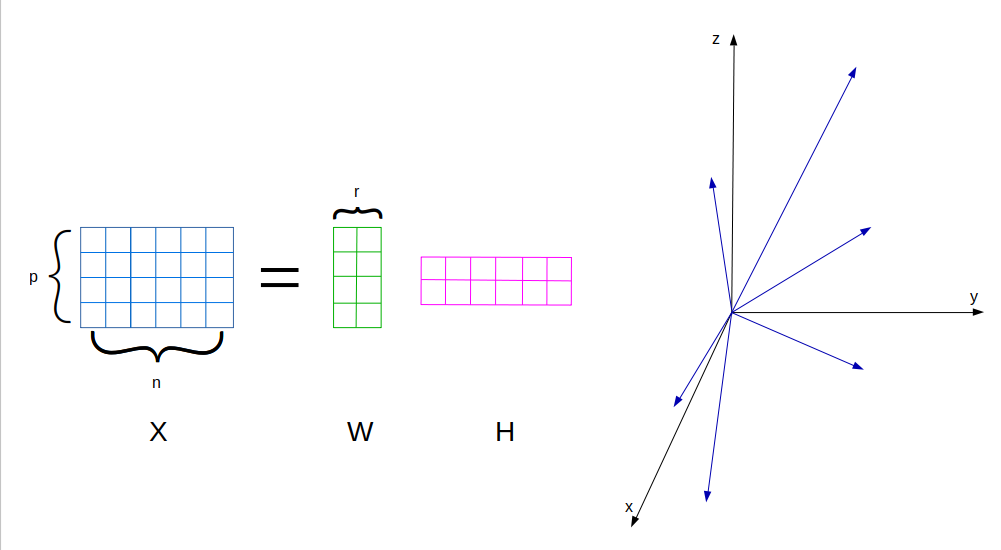
\includegraphics[scale=0.28]{../images/NMFvect.png}
\end{frame}
\begin{comment}
\begin{frame}{Computational Geometry : Nested polytopes problem}
\begin{figure}
\centering
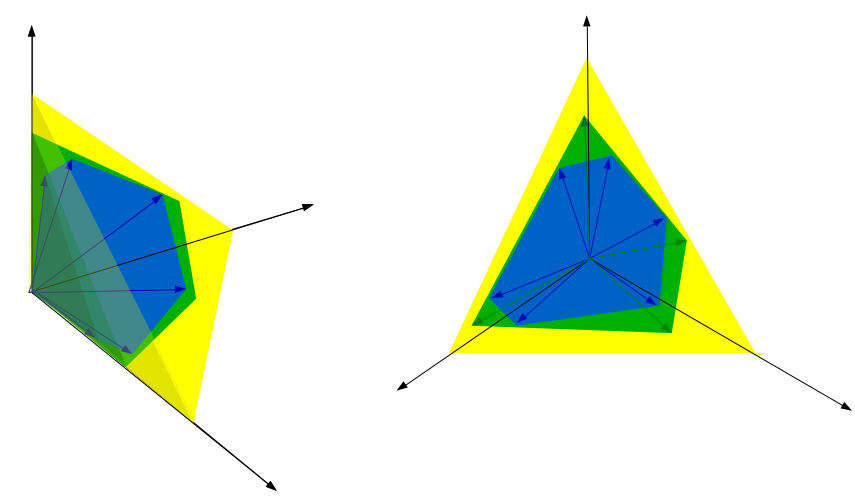
\includegraphics[scale=0.35]{../images/polytopeGeo.png}
\caption{\footnotesize Finding a polytope with minimum nb of vertices nested between 2 polytopes}
\end{figure}
\end{frame}
\end{comment}
\begin{frame}{Graph Theory : Bipartite dimension}
Let $G(X) = (V_1 \cup V_2, E)$ be a bipartite graph induced by X (i.e. $(i,j)\in E \Leftrightarrow X_{ij}\neq 0$).
\begin{defn}[Biclique and bipartite dimension]
\begin{itemize}
\item A biclique (or a complete bipartite graph) is a bipartite graph s.t. every vertex in $V_1$ is connected to every vertex in $V_2$. 
\item The bipartite dimension (or the minimum biclique cover) bc$(G(X))$ is the minimum number of bicliques needed to cover all edges in E.
\end{itemize} 
\end{defn}

\end{frame}

\begin{frame}

\begin{figure}
\centering
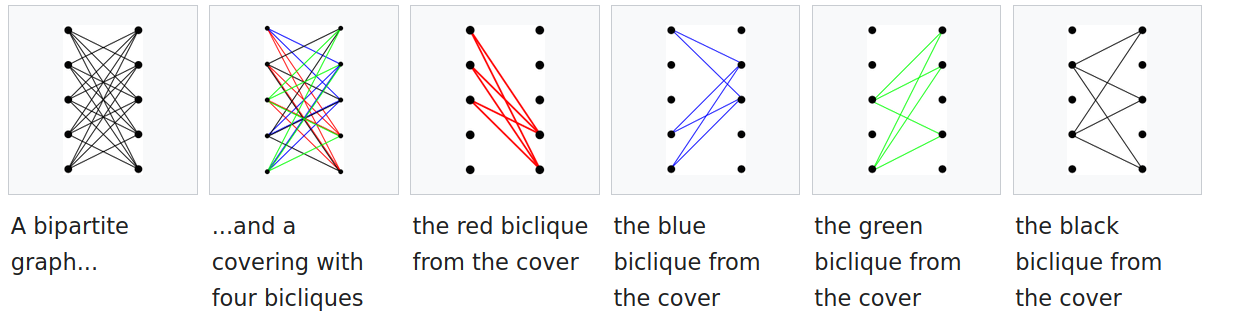
\includegraphics[scale=0.2]{../images/biclique.png}
\caption{Example for biclique edge cover \cite{biclique}}
\end{figure}
\begin{comment}
For any $(W,H)\geq 0$ s.t. $X = WH = \sum_{k=1}^r W_{:k}H_{k:} := \sum_{k=1}^r X_k$, we have 
\[G(X) = \cup_{k=1}^r G(W_{:k}H_{k:})
\]
where $G(W_{:k}H_{k:})$ are complete bipartite subgraphs (bc$(G(W_{:k}H_{k:}) = 1 \forall k$).
\end{comment}
\begin{thm}[Rectangle covering bound]
\[\text{bc}(G(X))\leq \text{rank}_+(X)
\]
\end{thm}
\end{frame}
\begin{comment}
\begin{frame}{Communication complexity}
\begin{center}
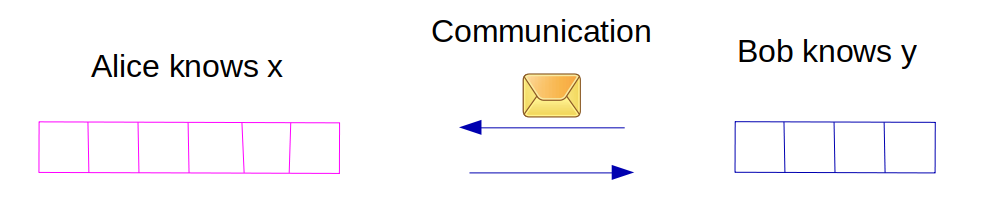
\includegraphics[scale=0.2]{../images/communication.png}
\end{center}
\small
Alice and Bob want to compute :
\[f:\{0,1\}^m \times \{0,1\}^n \rightarrow \{0,1\} : (x,y) \rightarrow f(x,y)
\]
While minimizing the nb of bits exchanged (i.e. communication complexity (CC)).


\textbf{Nondeterministic comm. complex. of $f$ (NCC)}: CC of $f$ with oracle/ message before starting the communication.


The communication matrix $X \in \{0,1\}^{2^n\times 2^m}$ is equal to the function $f$ for all possible combinations of inputs.

\begin{thm}[Yannakis]
\[\text{NCC of } f \leq \log_2(\text{rank}_+(X))
\]
\end{thm}
\end{frame}
\end{comment}
\begin{frame}{Linear Optimization : Extended formulation}
\begin{align*}
\text{(LP) } & \max & c^T x\\
 &s.t. & Ax\leq b\\
 & & x \in \mathbb{R}^n \geq 0
\end{align*}
\begin{defn}[Extended formulation]
The extended formulation of a polytope P is a higher dimensional polytope Q and a linear projection $\pi$ s.t. $\pi(Q) = P$.
\end{defn}
In our LP problem, an extended formulation of the polytope $P \subset \mathbb{R}^n$ defined by the constraints $Ax\leq b$, is a polytope $Q\subset \mathbb{R}^{n+r}$ defined by $Cx+Dy \leq d$ with $y\in \mathbb{R}^r$, s.t. $\pi(Q) = P$.

\end{frame}

\begin{frame}
The slack matrix $X(i,j) = b_i-A_iv_j$.

With $v_j$, the $j^{th}$ vertex of P and $\{x\in \mathbb{R}^n | b_i-A_ix\geq 0\}$ its $i^{th}$ facet.

The (i,j) entry measures the slack of the $i^{th}$ inequality for the $j^{th}$ vertex. 
\begin{thm}[Yannakis]
The minimum size of an extended formulation Q of P is equal to $\text{rank}_+(X)$.
\end{thm}

When P has exponentially many facets, finding extended formulations allows to solve the LP in polynomial time.
\end{frame}
	\section{Conclusion}
  	\begin{frame}{Conclusion}
  	\centering
  	{\huge Thanks for listening!}
  	
  	\vspace{2cm}
  	
  	{\Large Any questions?}
  	\end{frame}
  	
\end{document}
